\chapter{Aplicação a dados da amostra de Vredefort}
\label{sec:lab_application}

Uma cratera de impacto é o registro de um dos processos geológicos mais rápidos já conhecidos. As altas pressões ($> 5$ GPa) e as altas temperaturas ($> 1000^\circ$C) de choque são responsáveis pela formação de sistemas geoquímicos únicos. A evolução de tais sistemas podem gerar assinaturas petrofísicas complexas \citep{pilkington_grieve_1992,pilkington_hildebrand_2003,yokoyama_etal_2015}. Um exemplo destas assinaturas pode ser observado em dados magnéticos do domo de Vredefort, na África do Sul. O domo de Vredefort é uma das mais extensas estruturas de impacto já conhecida na Terra, com um diâmetro de aproximadamente $250$ km, de forma que estudos magnéticos tem sido realizados desde os anos 60. Esta estrutura possui diversos tipos de impactitos, tais como veios de impacto, diques com estrutura granofírica e \textit{shatter cones}. Neste contexto, estudos paleomagnéticos são recorrentes em veios de impactos, especialmente os pseudotaquilitos. Estas rochas são escuras e vítreas formadas, principalmente, por forte fricção. Elas são encontradas em zonas de falha e cisalhamentos, e em algumas estruturas de impacto tais como o domo de Vredefort. Portanto, neste trabalho, foi utilizada uma amostra da região de Leeukop Quarry no domo de Vredefort \citep{araujo_etal2019_materials}, similar às usadas em outros estudos paleomagnéticos \citep{passchier_1982,lana_etal_2003,dressler_reimold_2004,carporzen_etal_2005,araujo_etal2019_sensors}. Na Figura \ref{fig:datafit_real_sample}a apresentamos o mapa de microscopia magnética da amostra de Vredefort. Estas medidas foram realizadas em ambiente com blindagem para campos magnéticos de até $15$ mT. Além disso, aplicamos um campo magnético de $400$ mT na direção do eixo $z$. Os dados foram medidos em um grid regular de $121 \times 99$ pontos (um total de $N=11979$ observações) sobre uma área que se estende em $36$ mm e $30$ mm ao longo dos eixos $x$ e $y$, respectivamente. A distância sensor-amostra foi igual a $138 \, \mu$m acima da superfície da amostra. 


Para a inversão, utilizamos uma camada equivalente formada por um grid de $121 \times 99$ dipolos (um total de $M=11979$ fontes equivalentes) posicionadas a uma profundidade constante de $z_c = 818 \, \mu$m abaixo da superfície de observação. A direção de magnetização para os dipolos é igual a $90^\circ$ para a inclinação e $0^\circ$ para a declinação, que é a mesma direção do campo aplicado na amostra. Resolvendo a equação \ref{eq:linear_sys_p_alpha}, estimamos a distribuição de momentos magnéticos sobre a camada equivalente (não mostrado). A figura \ref{fig:datafit_real_sample}b mostra os dados preditos produzidos pela camada equivalente. Na figura \ref{fig:datafit_real_sample}c é apresentado o mapa dos resíduos, que é definido como a diferença entre os dados observados (Figura \ref{fig:datafit_real_sample}a) e os dados preditos (Figura\ref{fig:datafit_real_sample}b). O histograma dos resíduos aparece com média de $0$ mT e desvio padrão de $0,03$ mT (Figura \ref{fig:datafit_real_sample}d). Isto significa que a distribuição de momentos magnéticos produziu um ajuste aceitável dos dados observados. As componentes e a amplitude do campo magnético preditas pela camada equivalente são mostradas nas figuras \ref{fig:components_real_sample}a, \ref{fig:components_real_sample}b, \ref{fig:components_real_sample}c e \ref{fig:components_real_sample}d. O resultado apresentado na figura \ref{fig:components_real_sample}d mostra uma concentração de minerais magnéticos na borda superior da amostra de Vredefort. Com os resultados apresentados, podemos concluir que a técnica da camada equivalente pode ser uma ferramenta útil para o processamento de dados magnéticos, de forma que conseguimos calcular as componentes do campo magnético e sua amplitude sem termos conhecimento prévio da direção de magnetização da fonte magnética. 

%%% Figuras para aplicação a dados reais 
\begin{figure}
	\centering
	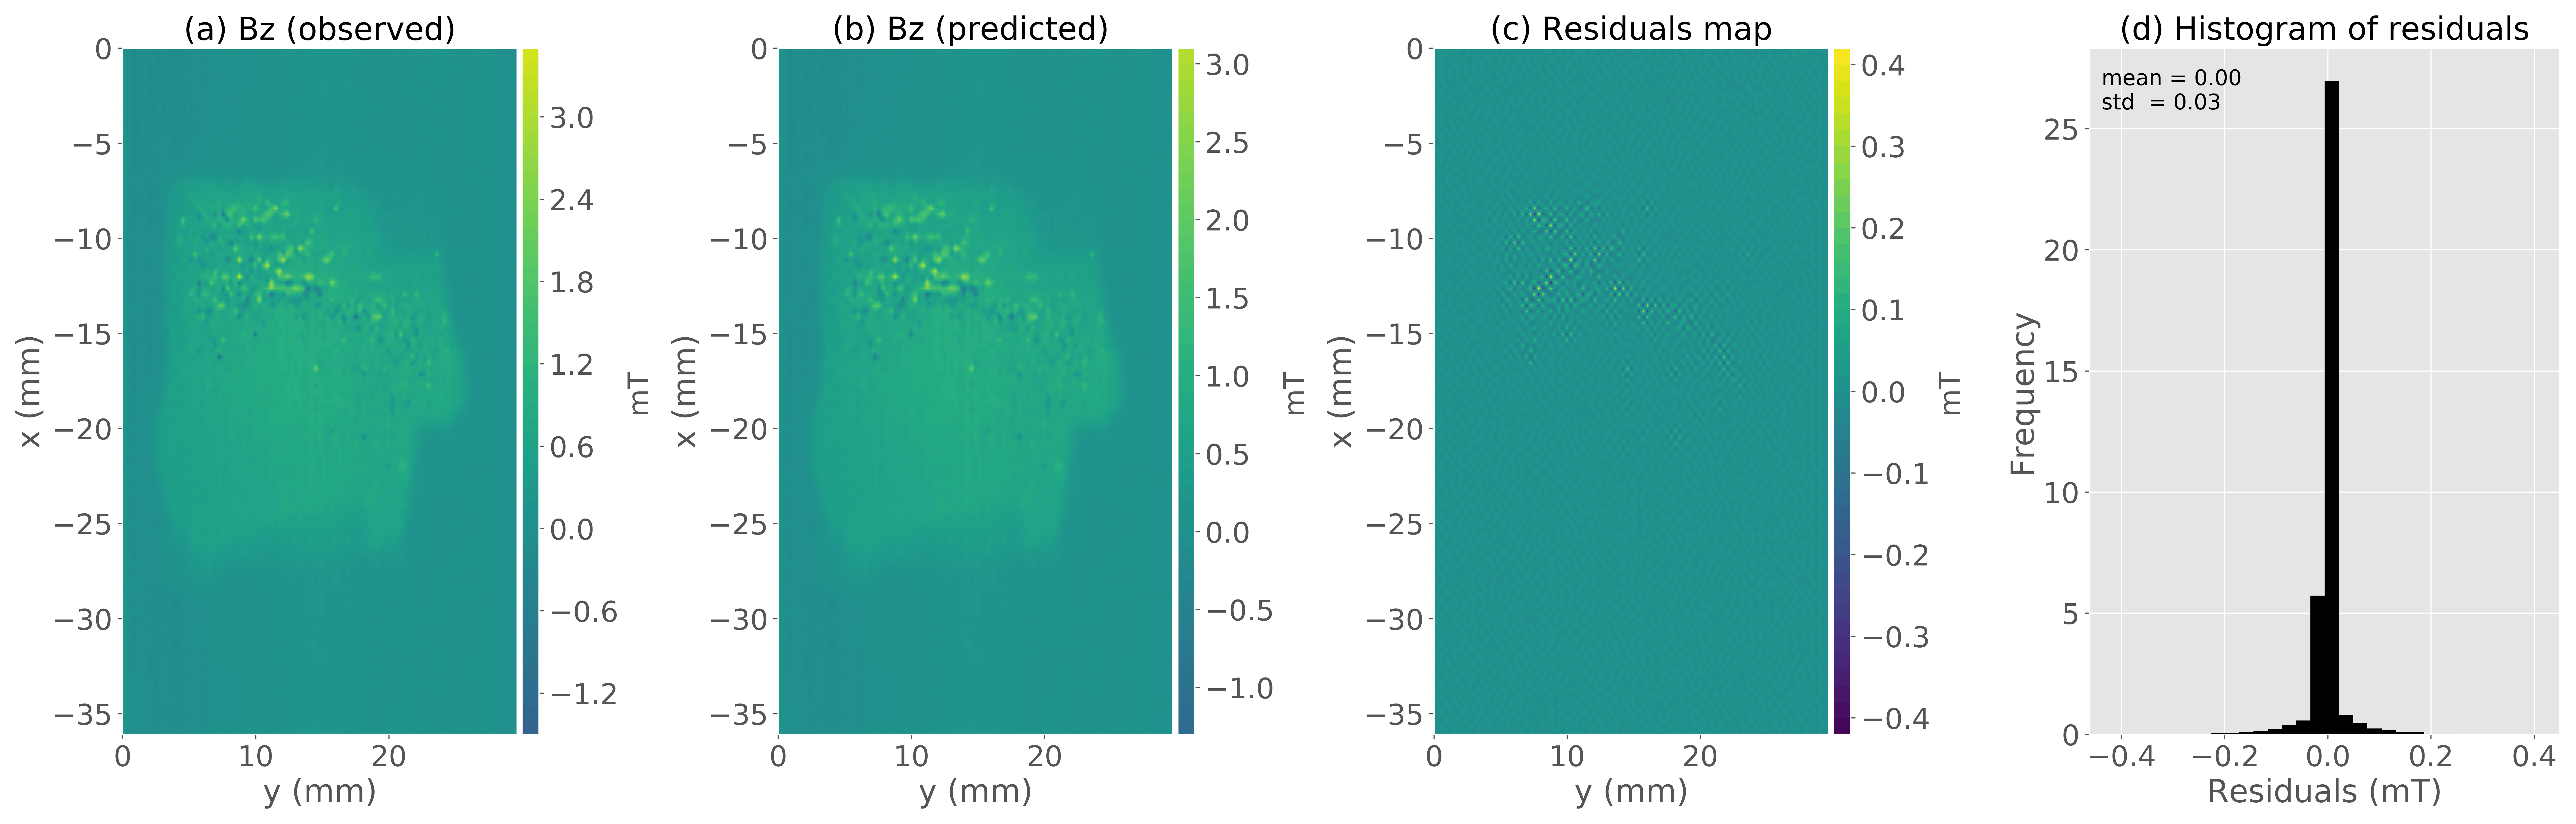
\includegraphics[width=.9\textwidth]{Fig/mag_vec/aplicacao_vredefort/results_data_fitting_Bz.png}
	\caption{Aplicação a dados de laboratório para a amostra de Vredefort \citep{araujo_etal2019_materials}. (a) Componente vertical observada. (b) Dados preditos produzido pela camada equivalente. (c) Diferença entre os dados mostrados nos gráficos a e b. (d) Histograma dos resíduos.}
	\label{fig:datafit_real_sample}
\end{figure}

\begin{figure}
	\centering
	\includegraphics[width=1.\textwidth]{Fig/mag_vec/aplicacao_vredefort/field_components_eqlayer.png}
	\caption{Aplicação a dados de laboratório para a amostra de Vredefort \citep{araujo_etal2019_materials}. (a) Componente vertical predita pela camada. (b) Componente $x$ do campo magnético predita pela camada. (c) Componente $y$ do campo magnético predita pela camada. (d) Amplitude do campo magnético calculado através da equação \ref{eq:amplitude_field}.}
	\label{fig:components_real_sample}
\end{figure}

